\documentclass[t]{beamer}
\setbeamertemplate{theorems}[numbered]
\setbeamertemplate{navigation symbols}{}
\usetheme{Frankfurt}
\usepackage{mathtext}          
\usepackage[T2A]{fontenc}          
\usepackage[utf8]{inputenc}         
\usepackage[english,russian]{babel} 
\usepackage{comment}
\newtheorem{myth}{Теорема}
\newtheorem{mylm}{Лемма}
\newtheorem*{myco}{Следствие}
\usepackage{amsmath,amsfonts,amssymb,amsthm,mathtools}
\usepackage{icomma}
\newcommand{\pphi}[1] {P^{\delta}(\varphi_{#1})}
\usepackage{graphicx}

\title{О длине некоторых периодических функций пятизначной логики в классе поляризованных
    полиномиальных форм}
\author{Михаил Гордеев}
\date{\today}
\institute[МГУ]{МОСКОВСКИЙ ГОСУДАРСТВЕННЫЙ УНИВЕРСИТЕТ \\
    Факультет Вычислительной Математики и Кибернетики}

\begin{document}

\frame[plain]{\titlepage}

\section{Введение}
\begin{frame}
\frametitle{\insertsection}
В данной работе рассматривается класс функций $\mathcal{A}$, состоящий из всех линейных комбинаций
функций $f$ и $g$, где $f$ -- это периодическая симметрическая функция с периодом (1,1,4,4), а
\mbox{$g$ -- это} периодическая симметрическая функция с периодом (1,4,4,1). А также его подкласс
$\mathcal{F}$ состоящий из следующих четырех функций: $f,g,f+g,f+4g$.
\end{frame}

\section{Основные теоремы и леммы}
\subsection{Длина функций $s^2$ и $s^3$}
\begin{frame}
\frametitle{\insertsection}
\framesubtitle{\insertsubsection}
\begin{myth}
\label{ths}
При $n \geqslant 1$ и $s_n$ любой из функций ${s^2_n = f_n + 2\,g_n}$, ${s^3_n = f_n + 3\,g_n}$
длина полинома периодической функции пятизначной логики~$s_n$
при поляризации $\delta = (d_1,\ldots,d_n)$выражается следующей формулой:
$$ l(P^{\delta}(s_n)) = 5^{n-m} \cdot 4^m ,$$
где $m = \begin{cases}
\text{количество } 4 \text{ в векторе } \delta, \text{ если } s_n = s^2_n; \\
\text{количество } 2 \text{ в векторе } \delta, \text{ если } s_n = s^2_n.
\end{cases}$
\end{myth}
\end{frame}

\subsection{Нижняя оценка}
\begin{frame}
\frametitle{\insertsection}
\framesubtitle{\insertsubsection}
\only<1> {
\begin{mylm}
При векторе поляризации $\delta = (d_1,\dots,d_n), d_i \in \{0,1,3,4\}, i = 1,\dots,n$ и
$\varphi_n$ -- любой функции из $\mathcal{F}^n$ верно:
$$l(\pphi{n}) \geqslant \frac{2}{5} \cdot 5^n.$$
\end{mylm}
\begin{mylm}
\label{lm24l}
При векторе поляризации $\delta=(d_1,\dots,d_n),\ d_i = 2,\ i=1,\dots,m,\ d_i=4,{\ i=n-m+1,\dots,n}$
и $\varphi_n$ -- любой функции из $\mathcal{F}^n$ верно:
$$l(\pphi{n})\geqslant\left(\left(\frac{5}{4}\right)^m-\frac{3}{2}\right)\cdot4^n+4^m\cdot5^{n-m}.$$
\end{mylm}
}
\only<2> {
\begin{myth}
При векторе поляризации $\delta=(d_1,\dots,d_n)$ и $\varphi_n$ -- любой функции из
$\mathcal{F}^n$ верно: $$l(\pphi{n}) \geqslant \left(\left(\left(\frac{5}{4}\right)^{m_2}-
\frac{3}{2}\right) \cdot 4^{m_2+m_4}+4^{m_2}\cdot 5^{m_4} \right) \cdot 5^{n-m_2-m_4},$$
где $m_2$ -- число $2$ в $\delta$, а $m_4$ -- число $4$.
\end{myth}
}
\end{frame}

\subsection{Верхняя оценка}
\begin{frame}
\frametitle{\insertsection}
\framesubtitle{\insertsubsection}
\begin{myth}
\label{thh}
Для любой функции $\varphi_n$ из $\mathcal{F}^n$, при $n$ четном верно:
$$ l(\varphi_n) \leqslant 4^n\left( 2 \cdot \left (\frac{5}{4} \right)^{\frac{n}{2}} - 1 \right).$$
\end{myth}
\begin{myco}
Класс функций $\mathcal{A}$ является вырожденным.
\end{myco}
\end{frame}

\section{Результаты}
\subsection{Математические результаты}
\begin{frame}
\frametitle{\insertsection}
\framesubtitle{\insertsubsection}
\begin{enumerate}
\item Для всех функций из класса $\mathcal{A}$ были построены построены все поляризованные
полиномы, выражающие функции от $n+1$ переменных через функции от $n$ переменных также принадлежащих
классу $\mathcal{A}$;
\item<2-> Установле точная длина, в зависимости от поляризации, для функций: $s^2_n$ и $s^3_n$;
\item<3-> Доказано несколько теорем и лемм, из которых получается нижняя оценка для функций из
класса $\mathcal{F}$;
\item<4-> Установлена верняя оценка для функций из класса $\mathcal{F}$;
\item<5-> Доказана вырожденность класса $\mathcal{A}$.
\end{enumerate}
\end{frame}

\subsection{Программные результаты}
\begin{frame}
Для получения результатов были написаны следующие программы:
\frametitle{\insertsection}
\framesubtitle{\insertsubsection}
\only<1> {
\begin{itemize}
\item Программа на языке \ttfamily{C++}, реализующая построение поляризованных полиномов по
    модулю~$k$, где $k \in {2,3,5,7}$;
\item Для этой программы был написан интерфейс на языке \ttfamily{Perl}, передставленный на
    рисунке;
    \begin{figure}[h]
    \centering
    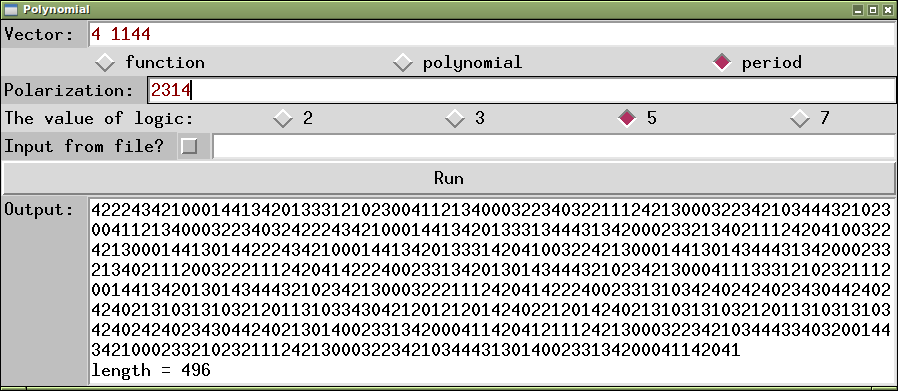
\includegraphics[width=0.65\textwidth]{polyscreen.png}
    \end{figure}
\end{itemize}
}
\only<2> {
\begin{itemize}
\item Программа на языке \ttfamily{C++}, осуществляющая для заданного числа пременных $n$
    "быстрый"{} поиск функций длина которых, в классе пляризованных полиномов, больше заданного
    порога, среди заданного класса симметрических функций от $n$ переменных;
\item С помощью системы компьютерной алгебры \ttfamily{Sage} были произведены: получение
    полиномиальных форм, поляризованных по разным векторам поляризации и подстановка значений в
    полиномы для проверки правильности их построения.
\end{itemize}
}
\end{frame}
\end{document}
